% Standalone TikZ drawing of the region \mathcal{T} of Definition 4.21 of
% finite_contour_cocycles_short.tex, superimposed on the fundamental domain
% \mathcal{F}, its S-image S\mathcal{F}, and their T-translates.
%
%   \mathcal{T} = { 0 <= Re t <= 1, 1/2 <= Im t <= 1, |t-i/2| >= 1/2, |t-1-i/2| >= 1/2 }
%
% Compile standalone:   pdflatex T_region.tex
% Or \input directly inside a figure environment in the note.
\documentclass[border=8pt]{standalone}
\usepackage{lmodern}
\usepackage{amsmath,amssymb}
\usepackage{tikz}
\usetikzlibrary{arrows.meta}

\definecolor{Ffill}{HTML}{DCE7F2}\definecolor{Fline}{HTML}{7F9AB4}
\definecolor{Sfill}{HTML}{DFEEDD}\definecolor{Sline}{HTML}{7BA475}
\definecolor{Tfill}{HTML}{F0A860}\definecolor{Tline}{HTML}{A8410A}
\definecolor{Gline}{HTML}{1F4E79}

\begin{document}
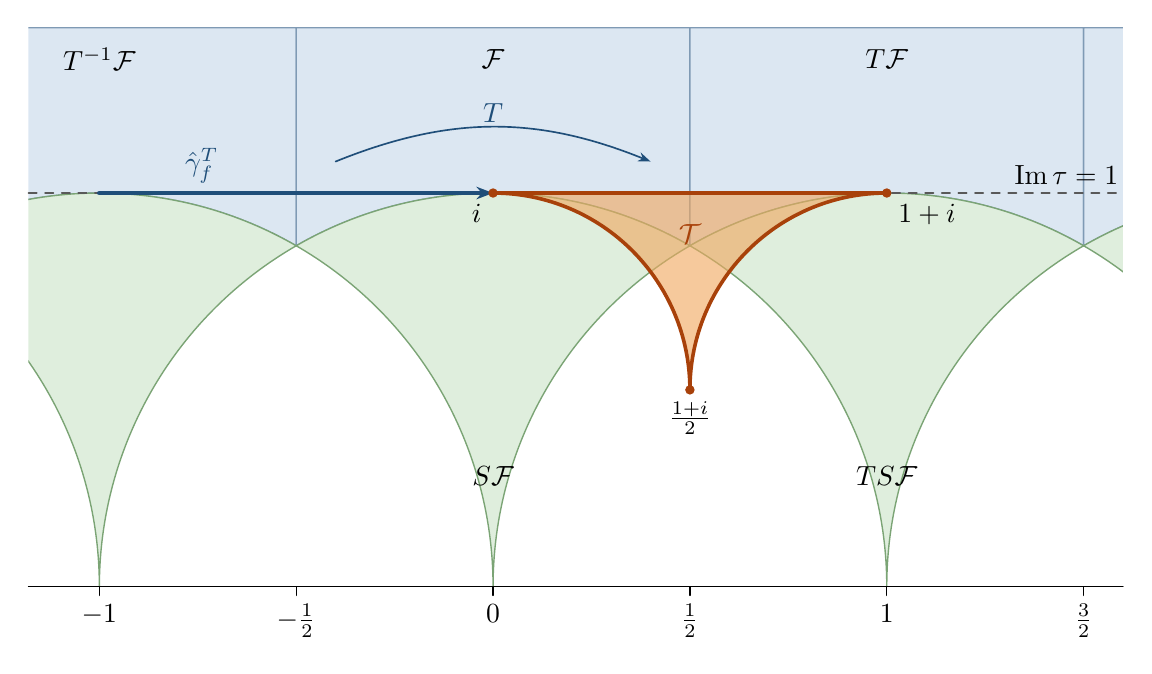
\begin{tikzpicture}[scale=5,line join=round,line cap=round]
\def\ytop{1.42}
\def\xa{-1.18}
\def\xb{1.60}
\def\rh{0.86602540378}          % Im(rho) = sqrt(3)/2

% ---- tiling: F and S.F, with T-translates, clipped to the window ----
\begin{scope}
  \clip (\xa,0) rectangle (\xb,\ytop);
  \foreach \dx in {-1,0,1,2}{\begin{scope}[shift={(\dx,0)}]
      \fill[Ffill,draw=Fline,line width=0.5pt]
        (-0.5,\ytop) -- (-0.5,\rh)
        arc[start angle=120, end angle=60, radius=1]
        -- (0.5,\ytop) -- cycle;
  \end{scope}}
  \foreach \dx in {-1,0,1,2}{\begin{scope}[shift={(\dx,0)}]
      \fill[Sfill,draw=Sline,line width=0.5pt]
        (-0.5,\rh)
        arc[start angle=120, end angle=60,  radius=1]   % |t|=1
        arc[start angle=120, end angle=180, radius=1]   % |t-1|=1
        arc[start angle=0,   end angle=60,  radius=1];  % |t+1|=1
  \end{scope}}
\end{scope}

% ---- the T-segment of the reference contour ----
\draw[dashed,gray!70!black,line width=0.6pt] (\xa,1) -- (\xb,1);
\node[anchor=south east,inner sep=1.5pt] at (\xb,1.01) {$\operatorname{Im}\tau=1$};

% ---- the region T itself ----
\fill[Tfill,opacity=0.62]
  (0,1) -- (1,1)
  arc[start angle=90, end angle=180, radius=0.5]        % |t-1-i/2|=1/2
  arc[start angle=0,  end angle=90,  radius=0.5];       % |t-i/2|=1/2
\draw[Tline,line width=1.3pt]
  (0,1) -- (1,1)
  arc[start angle=90, end angle=180, radius=0.5]
  arc[start angle=0,  end angle=90,  radius=0.5];

% ---- real axis ----
\draw[line width=0.5pt] (\xa,0) -- (\xb,0);
\foreach \t/\l in {-1/{-1}, -0.5/{-\tfrac12}, 0/{0}, 0.5/{\tfrac12}, 1/{1}, 1.5/{\tfrac32}}{
  \draw[line width=0.5pt] (\t,0) -- (\t,-0.022);
  \node[anchor=north,inner sep=3pt] at (\t,-0.022) {$\l$};}

% ---- the reference T-segment itself, and the translate that caps T ----
\draw[Gline,line width=1.7pt,-{Stealth[length=6pt]}] (-1,1) -- (0,1);
\node[Gline,anchor=south,inner sep=3.5pt] at (-0.74,1) {$\hat\gamma^T_f$};
\draw[Gline,line width=0.6pt,-{Stealth[length=4.5pt]}]
  (-0.40,1.08) to[bend left=22]
  node[midway,above,inner sep=1.5pt,text=Gline]{$T$} (0.40,1.08);

% ---- region labels ----
\node at (-1,1.34) {$T^{-1}\mathcal{F}$};
\node at (0,1.34)  {$\mathcal{F}$};
\node at (1,1.34)  {$T\mathcal{F}$};
\node at (0,0.28)  {$S\mathcal{F}$};
\node at (1,0.28)  {$TS\mathcal{F}$};
\node[Tline] at (0.5,0.895) {$\mathcal{T}$};

% ---- marked points: the three vertices of T ----
\foreach \x/\y/\l/\a in {%
    0/1/{i}/{north east},
    1/1/{1+i}/{north west},
    0.5/0.5/{\tfrac{1+i}{2}}/{north}}{
  \fill[Tline] (\x,\y) circle[radius=0.012];
  \node[anchor=\a,inner sep=4pt] at (\x,\y) {$\l$};}
\end{tikzpicture}
\end{document}
